\documentclass[tikz,margin=0mm]{standalone}

\usepackage[utf8]{inputenc}
\usepackage{amsmath}
\usepackage[default]{opensans}
\usepackage{stix}

\usepackage{pgfplots}
\usepackage{tikzlings}
\usepackage{moeptikz}
\usepgfplotslibrary{statistics}
\pgfplotsset{compat=1.18}
\usetikzlibrary{positioning,fit,3d,decorations.markings,shapes}

\begin{document}

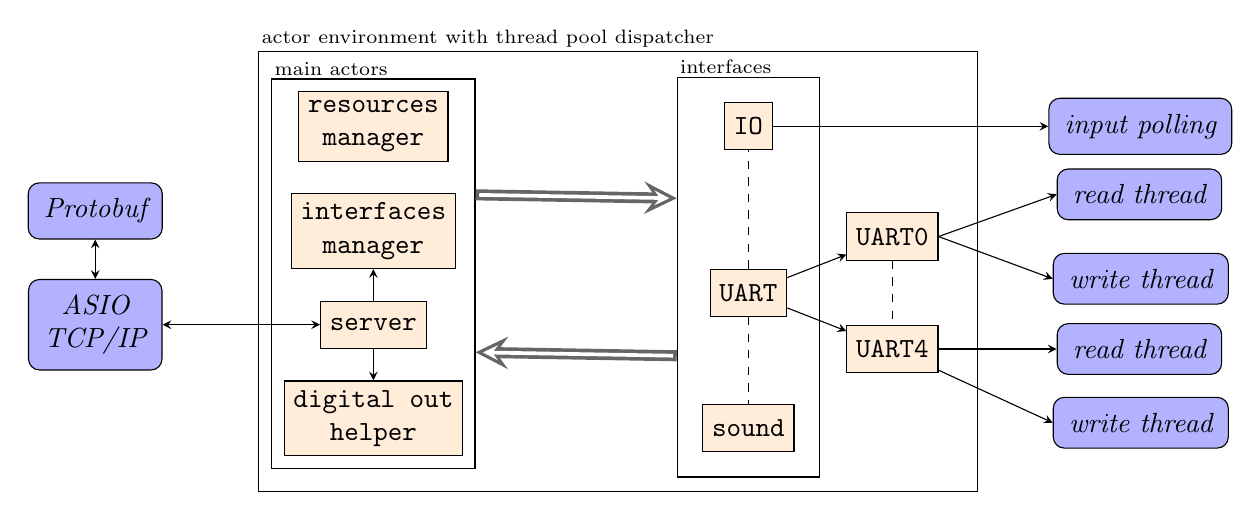
\begin{tikzpicture}[>=stealth,
    nonactor/.style={
        rectangle,
        rounded corners,
        draw=black,
        minimum width=1cm, minimum height=4mm,
        inner sep=2mm,
        text centered,
        align=center,
        fill=blue!30,
        font=\itshape
        },
    actor/.style={
    % The shape:
        rectangle,
        minimum size=6mm,
        % The rest
        %very thick,draw=black!50,
        draw=black,
        fill=orange!15,
        align=center,
        font=\ttfamily},
    double arrow/.style args={#1 colored by #2 and #3}{
            -stealth,line width=#1,#2, % first arrow
            postaction={draw,-stealth,#3,line width=(#1)/3,
                        shorten <=(#1)/3,shorten >=2*(#1)/3}, % second arrow
        }]
    
    
    \node (res_man) [actor] {resources\\manager};
    \node (int_man) [actor, below=0.4cm of res_man] {interfaces\\manager};
    \node (server) [actor, below=0.4cm of int_man] {server};
    \node (dig_out) [actor, below=0.4cm of server] {digital out\\helper};
    
    \node (io) [actor, right=3.5cm of res_man] {IO};
    \node (uart) [actor, below=1.5cm of io] {UART};
    \node (sound) [actor, below=1.1cm of uart] {sound};

    \node (uart0) [actor, above right=0.1cm and 0.75cm of uart] {UART0};
    \node (uart4) [actor, below right=0.1cm and 0.75cm of uart] {UART4};

    \node (uart_read0) [nonactor, above right=-0.1 and 1.5cm of uart0] {read thread};
    \node (uart_write0) [nonactor, below right=-0.1 and 1.45cm of uart0] {write thread};

    \node (uart_read4) [nonactor, right=0 and 1.5cm of uart4] {read thread};
    \node (uart_write4) [nonactor, below right=0.3cm and 1.45cm of uart4] {write thread};

    \node (io_pool) [nonactor, right=3.5cm of io] {input polling};

    \node (boost_asio) [nonactor, left=2cm of server] {ASIO\\TCP/IP};
    \node (protobuf) [nonactor, above=0.5cm of boost_asio] {Protobuf};

    \node[draw=black, inner sep=1ex, fit={(res_man)(dig_out)}] (fit_main) {};
    \node[above right, inner sep=1pt, font=\scriptsize] at (fit_main.north west) {main actors};

    \node[draw=black, inner sep=1ex, inner sep=0.318cm, fit={(io)(sound)}] (fit_int) {};
    \node[above right, inner sep=1pt, font=\scriptsize] at (fit_int.north west) {interfaces};

    \node[draw=black, inner sep=1ex, inner sep=0.5cm, fit={(res_man)(sound)(uart4)}] (fit_act) {};
    \node[above right, inner sep=1pt, font=\scriptsize] at (fit_act.north west) {actor environment with thread pool dispatcher};

    \path (server) edge[->] (dig_out);
    \path (server) edge[->] (int_man);

    \path (uart0) edge[dashed] (uart4);
    \path (uart) edge[->] (uart0);
    \path (uart) edge[->] (uart4);
    
    \path (uart) edge[dashed] (io);
    \path (uart) edge[dashed] (sound);

    \draw[->] (uart0.east) -- (uart_read0.west);
    \draw[->] (uart0.east) -- (uart_write0.west);
    \path (uart4) edge[->] (uart_read4);
    \path (uart4) edge[->] (uart_write4.west);

    
    \path (io) edge[->] (io_pool);
    
    
    \path (server) edge[<->] (boost_asio);
    \path (boost_asio) edge[<->] (protobuf);

    \draw[double arrow=4pt colored by black!60!white and white, transform canvas={yshift=1cm}] (fit_main.east) -- (fit_int.west);
    \draw[double arrow=4pt colored by black!60!white and white, transform canvas={yshift=-1cm}] (fit_int.west) -- (fit_main.east);
    %\draw[<->, thick] (fit_main.east) -- (fit_int.west);
    %\draw[<->, thick, transform canvas={yshift=1.8cm}] (fit_main.east) -- (fit_int.west);
    %\draw[<->, thick, transform canvas={yshift=-1.8cm}] (fit_main.east) -- (fit_int.west);

    %\draw[<->] (res_man.east) -- (io);
    %\draw[->] (res_man.east) ++(2.5cm,0) |- (uart.west);
    %\draw[->] (res_man.east) ++(2.5cm,0) |- (sound.west);

    %\draw[<->] (server.east) -- ++(2.2cm,0) |- (uart.south west);
    %\draw[->] (server.east) ++(2.2cm,0) |- (io.south west);
    %\draw[->] (server.east) ++(2.2cm,0) |- (sound.south west);

    %\draw[<->] (dig_out.east) -- ++(1.2cm,0) |- (uart.north west);
    %\draw[<->] (dig_out.east) -- ++(1.2cm,0) |- (io.base west);
    %\draw[->] (dig_out.east) ++(1.2cm,0) |- (sound.base west);

    %\draw[->] (int_man.east) -- ++(0.8cm,0) |- (uart.north west);
    %\draw[->] (int_man.east) ++(0.8cm,0) |- (io.north west);
    %\draw[->] (int_man.east) ++(0.8cm,0) |- (sound.north west);
\end{tikzpicture}

\end{document}